\documentclass[aps,pre,twocolumn,superscriptaddress,amsmath,amssymb,10pt]{revtex4-2}
\usepackage{graphicx}
\usepackage{bm}
\usepackage[colorlinks=true,linkcolor=blue,citecolor=blue,urlcolor=blue]{hyperref}

\newcommand{\Lc}{\mathcal{L}}
\newcommand{\J}{\mathcal{J}}
\newcommand{\tr}{\operatorname{tr}}

\begin{document}

\title{Energy mode versus two-fermion continuum: slow-mode competition in the Lindbladian of the dissipative Sachdev-Ye-Kitaev model}

\author{[Author]}
\affiliation{[Affiliation]}

\date{\today}

\begin{abstract}
The Lindbladian of the Sachdev-Ye-Kitaev (SYK) model with linear Majorana jump operators of strength $\mu$ has the Hamiltonian $H$ as an exact eigenoperator with decay rate $q\mu$ [Garc\'ia-Garc\'ia \emph{et al.}, Phys.\ Rev.\ E \textbf{113}, 024116 (2026)]. We ask when this energy mode sets the spectral gap of the physical, parity-even operator space. This addresses two points left open in earlier work: the relation between the finite-$N$ gap $4\mu$ and the large-$N$ decay rate of fermion correlations, and the expectation that conservation laws spoil anomalous relaxation. We separate a slow sector of energy-diagonal operators from a fast sector of coherences. In the slow sector, exact diagonalization (ED) for $N\le24$ shows that $H$ is the slowest mode and the next secular mode is faster by a factor that grows with $N$. In the fast sector, first-order perturbation theory gives rates $N\mu/2$ at finite $N$, whereas the large-$N$ two-fermion threshold $2\Gamma_1$ stays finite as $\mu\to0$. We then solve the large-$N$ Bethe-Salpeter equation for the four-point function on the doubled contour. The singlet ladder reproduces the energy mode as a bound state at $E=q\mu$, to within $10^{-3}$ relative accuracy for $0.05\le\mu/J\le0.3$. In the region we resolve, we find no other singlet or non-singlet bound state below $2\Gamma_1$. For $q=4$ this gives a gap transition at $\mu_c=0.323J$, where $q\mu_c=2\Gamma_1(\mu_c)$, and an analogous transition for $q=8$. ED with explicit mode identification gives a crossing that moves from $0.086J$ ($N=10$) to $0.184J$ ($N=18$). We explain the slow finite-size convergence by the crossover of the fast branch from $N\mu/2$ to $2\Gamma_1$. We also show where the picture fails: it does not hold for $N\le8$, and it does not apply to spin chains with lower-weight conservation laws.
\end{abstract}

\maketitle

\section{Introduction}

The asymptotic relaxation rate of a Markovian open quantum system is set by the spectral gap $\Delta$ of its Lindbladian~\cite{Kessler2012,Minganti2018}. For chaotic many-body systems, the weak-dissipation limit of $\Delta$ can be singular if one takes $N\to\infty$ first. This gives a finite ``anomalous'' relaxation rate, which has been related to quantum Ruelle-Pollicott resonances~\cite{Prosen2002,Mori2024,Jacoby2025,Zhang2026}. The SYK model~\cite{SY1993,Kitaev2015,MS2016} with linear jump operators $L_i=\sqrt\mu\,\psi_i$ is a solvable example. Its fermion Green's function decays at a rate $\Gamma_1$ that remains finite as $\mu\to0$~\cite{Kulkarni2022,Garcia2023}. The Keldysh contour of this model maps onto a two-site non-Hermitian SYK model with a wormhole-like dual~\cite{Garcia2023,MQ2018}.

Conserved quantities change this picture~\cite{Mori2024,Yang2025}. A conserved operator that is also an eigenvector of the dissipator decays at a rate independent of the dynamics~\cite{Teretenkov2024}. In the SYK model this is exact: $H$, the parity $P$ and $PH$ are simultaneous eigenvectors of the Hamiltonian and dissipative parts of the Lindbladian, with rates $q\mu$, $N\mu$ and $(N-q)\mu$~\cite{Garcia2026}. Finite-$N$ ED at small $\mu$ correspondingly shows a gap $4\mu$ for $q=4$ and $N>8$~\cite{Garcia2023}. Reference~\cite{Garcia2023} left open ``a more precise understanding of the relation between the spectral gap $\Delta$ and the decay rate'' of the Green's function. In random open quantum circuits, Ref.~\cite{Yoshimura2024} argued that conservation laws would spoil anomalous relaxation and deferred a systematic study. Earlier, Ref.~\cite{Cai2013} showed that a conserved magnetization makes the gap of a dissipative XXZ chain close. The exact energy mode makes the SYK model a natural place to quantify this effect.

These exact modes do not by themselves determine the gap. We address three questions. (i) Which modes compete with $H$, and for which $N$ is $H$ actually the slowest one? (ii) At large $N$, does any collective two-fermion mode lie below the threshold $2\Gamma_1$ set by a pair of single-fermion resonances? (iii) Where does the competition between the energy mode and the fast sector resolve, and how does the finite-$N$ answer approach the large-$N$ answer? Question (ii) requires the four-point ladder. The general ladder recursion on the Keldysh contour is known~\cite{Liu2026}, but for the dissipative SYK model it has so far been projected only onto out-of-time-order correlators to extract Lyapunov exponents~\cite{Garcia2024,Liu2026,Pelliconi2026}. Here we use the time-ordered sector, whose bound states are eigenvalues of the Lindbladian.

\section{Model, exact modes, and rigorous bounds}

We take $N$ Majorana fermions, $\{\psi_i,\psi_j\}=\delta_{ij}$, and $H=\sum_{i_1<\dots<i_q}J_{i_1\dots i_q}\psi_{i_1}\cdots\psi_{i_q}$ with $\overline{J^2_{i_1\dots i_q}}=J^2/\binom{N-1}{q-1}$ and $q\equiv0 \pmod 4$. This normalization gives the standard large-$N$ coupling $\J^2=qJ^2/2^{q-1}$. On parity-even operators the Heisenberg-picture Lindbladian is
\begin{equation}
\Lc(O)=i[H,O]-\mu\,\hat n(O),\qquad \hat n(O)=\tfrac N2O-\sum_i\psi_iO\psi_i,
\label{eq:L}
\end{equation}
where $\hat n$ multiplies a Majorana string by its length~\cite{Schuster2023,Bhattacharjee2023,Liu2024}. Since $\hat n$ is Hilbert-Schmidt Hermitian and $i[H,\cdot]$ is anti-Hermitian, every right eigenvector $X$ obeys $-\mathrm{Re}\,\lambda_X=\mu\,(X,\hat nX)/(X,X)$. This is a special case of the general statement that $\mathrm{Re}\,\lambda$ lies between the extreme eigenvalues of the Hermitian part of the Liouvillian~\cite{Barthel2022}. The smallest nonzero size of a traceless even operator is $2$. Combined with the exact mode $\Lc(H)=-q\mu H$~\cite{Garcia2026}, this gives
\begin{equation}
2\mu\le\Delta_N(\mu)\le q\mu
\label{eq:bound}
\end{equation}
for every $N$ and every disorder realization. The full gap therefore closes linearly in $\mu$, whatever order of limits is taken. The exact modes are simultaneously left and right eigenvectors, so they do not hybridize with the rest of the spectrum. For instance, $\mathrm{span}\{\openone,H\}^\perp$ is $\Lc$-invariant.

This does not guarantee that $H$ is the slowest mode, and the restriction $N>8$ noted in Ref.~\cite{Garcia2023} has a simple origin. For $N=6$ and $q=4$, the exact mode $PH$~\cite{Garcia2026} has rate $(N-q)\mu=2\mu$, and Eq.~\eqref{eq:bound} then forces $\Delta=2\mu$ for all $\mu$. We confirmed this numerically. For $N=8$ we find that $H$ is degenerate with the coherence sector at $\mu\to0$, and the gap is set by coherences for all $\mu>0$ (see below). Similarly, in spin models under uniform depolarizing noise of single-site rate $\gamma$, a two-body Hamiltonian is an eigenvector with rate $2\gamma$. A total magnetization conserved by the Hamiltonian, as in the XXZ chain, decays at $\gamma$, so in that case the energy mode never sets the gap. This is the mechanism behind the closing gap of the dissipative XXZ chain found in Ref.~\cite{Cai2013}. The question is therefore quantitative, and we now set up the decomposition needed to answer it.

\section{Slow and fast sectors}

At $\mu=0$ the kernel of $i[H,\cdot]$ consists of energy-diagonal operators. When the spectrum within each parity block is nondegenerate, this kernel has dimension $2^{N-1}$. We call it the slow sector $\mathcal S$; its orthogonal complement $\mathcal F$, the coherences, is the fast sector. Projecting out only $\openone$ and $H$ is not enough: all of $\mathcal S$ becomes slow for small $\mu$. Mori's projection removes the full energy-diagonal subspace for the same reason~\cite{Mori2024}, and the split is the weak-dissipation version of a metastable manifold~\cite{Macieszczak2016}. To first order in $\mu$, the rates are the eigenvalues of $\hat n$ restricted to each block of fixed Bohr frequency.

\emph{Slow sector.} On $\mathcal S$, first-order theory gives the secular generator $W_{EE'}=\sum_i|\langle E|\psi_i|E'\rangle|^2-\tfrac N2\delta_{EE'}$. Here $E$ is an exact eigenvector with eigenvalue $-q$. Numerically it is the slowest nonstationary eigenvector for all $10\le N\le24$, and the next eigenvalue $\lambda_2 q$ is separated from it [Fig.~\ref{fig:sectors}(a),(b)]. In units of $q\mu$, $\lambda_2$ grows from $1.04$ ($N=10$) to $1.81$ ($N=24$). The higher eigenvalues increase with $N$ as well. Their trend is consistent with the Ornstein-Uhlenbeck values $\lambda_k=k$, but we do not claim this limit. A controlled derivation would need concentration of $B=\sum_i[\psi_i,H]^\dagger[\psi_i,H]$, which enters through $\Lc(H^2)=-2q\mu H^2+\mu B$. Its relative fluctuation decreases as $N^{-0.81}$ for $10\le N\le20$ [Fig.~\ref{fig:sectors}(c)], which supports the approximation but does not prove it. For the gap, the relevant fact is only that the secular modes beyond $H$ are faster than $q\mu$ in the range we study.

\emph{Fast sector.} A coherence $|E\rangle\langle E'|$ with a nondegenerate Bohr frequency has first-order rate exactly $N\mu/2$. The reason is that $\psi_i$ is odd, so $\hat n$ couples such a coherence only to coherences of the opposite parity block, and generically none of those has the same frequency. Figure~\ref{fig:sectors}(a) confirms that for $N=12$ and $14$ the slowest fast mode has rate $N\mu/2$ to numerical precision. For $N=10$ ($N\equiv2 \pmod 8$) the two parity blocks have identical spectra. The resulting degenerate Bohr frequencies lower the rate to $\approx4.55\mu$, which is still above $q\mu$. For $N=8$ the fast rate $N\mu/2$ coincides with $q\mu$, and at small but finite $\mu$ the coherences become the slowest modes ($3.5$--$3.8\mu$ at $\mu=0.02J$). The energy mode is therefore the gap at weak dissipation only for $N\ge10$. In that regime the first-order fast rate $N\mu/2$ grows with $N$, whereas the large-$N$ fast branch saturates at a finite value (next section). The fast branch must interpolate between the two. This crossover is the source of the slow finite-size convergence discussed in Sec.~\ref{sec:muc}.

\begin{figure*}[t]
\centering
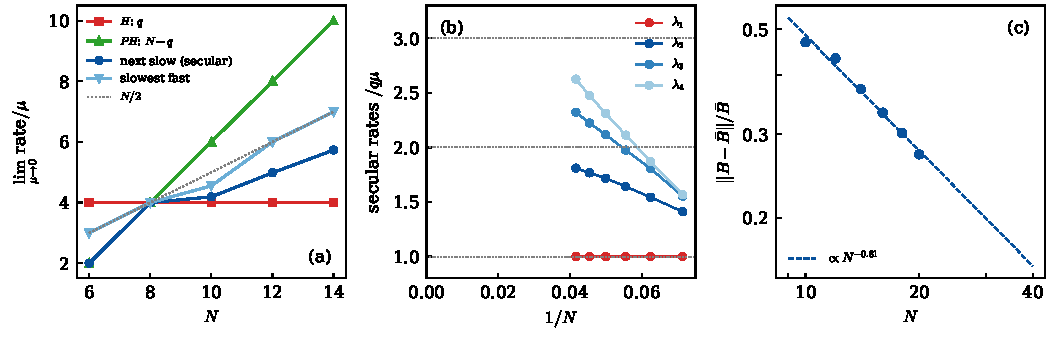
\includegraphics[width=\textwidth]{../figs/fig2_v2.pdf}
\caption{Slow and fast sectors at weak dissipation ($q=4$). (a) First-order ($\mu\to0$) rates in units of $\mu$: exact modes $H$ and $PH$, the slowest slow-sector mode other than $H$, and the slowest coherence (fast) mode. Three realizations are averaged; the scatter is smaller than the symbols. Dotted: $N/2$. (b) Secular eigenvalues $\lambda_k$ in units of $q\mu$; $\lambda_1=1$ is exact. (c) Relative Hilbert-Schmidt fluctuation of $B=\sum_i[\psi_i,H]^\dagger[\psi_i,H]$, which controls the closure of the energy-moment hierarchy.}
\label{fig:sectors}
\end{figure*}

\section{Large-$N$ two-fermion ladder}

Vectorizing $O\mapsto|O\rangle\!\rangle$ turns Eq.~\eqref{eq:L} into a two-site problem with fermions $\psi_{L}$ and $\psi_{R}$. The dissipator becomes $\mu N/2+i\mu\sum_i\psi_{L,i}\psi_{R,i}$, and the steady state $\openone$ becomes the ground state~\cite{Garcia2023}. Because all orders preserve the size grading, the $L$-$R$ Green's functions at large $N$ follow from the single function $C(t)=2^{-N/2}\tr[\psi_i(t)\psi_i]$:
\begin{equation}
G_{LL}=G_{RR}=\mathrm{sgn}(t)C(|t|),\qquad G_{LR}=-G_{RL}=iC(|t|).
\end{equation}
The function $C$ obeys the Kadanoff-Baym equation
\begin{equation}
\dot C=-\mu C-2^{2-q}J^2\!\int_0^t\!ds\,[2C(t-s)]^{q-1}C(s),
\label{eq:KB}
\end{equation}
with $C(0)=\tfrac12$. We checked Eq.~\eqref{eq:KB} against finite-$N$ Heisenberg evolution: the two agree to $2\times10^{-3}$ for $Jt\le3$ at $N=18$, $\mu=0$, and at $N=14$, $\mu=0.2J$. The single-fermion resonance $C\sim e^{z_1t}$ defines $\Gamma_1=-\mathrm{Re}\,z_1$. For $q=4$ we find $\Gamma_1(0)=0.630J$ and $\mathrm{Im}\,z_1(0)=0.385J$. The oscillation vanishes at an exceptional point $\mu_{\rm EP}\simeq0.16J$, in agreement with Ref.~\cite{Garcia2023}.

Even operators at leading order in $1/N$ are two-fermion states. A collective mode with decay rate $E$ appears as a normalizable solution of the Bethe-Salpeter equation $\Psi=K\Psi$. Following the Keldysh-contour recursion of Ref.~\cite{Liu2026}, the ladder kernel takes the standard form~\cite{MS2016,Garcia2024}
\begin{equation}
K_{ab,cd}=-(q-1)J^2c_cc_d\,G_{ac}(t_{13})G_{bd}(t_{24})G_{cd}(t_{34})^{q-2},
\end{equation}
with contour signs $c_{L}=-i$ and $c_{R}=+i$. We use the ansatz $\Psi_{ab}(t_1,t_2)=e^{-E(t_1+t_2)/2}\phi_{ab}(t_1-t_2)$. A bound state then corresponds to an eigenvalue $k(E)=1$ of a kernel acting on functions of the relative time on $[-S,S]$. Fermionic exchange, $\phi_{ab}(s)\to-\phi_{ba}(-s)$, splits the spectrum, as in the ladder of two coupled SYK models~\cite{Nosaka2020}. We keep only the antisymmetric sector, which is the physical one. The spurious symmetric solutions include one with $k(E)=1$ at $E\approx1.7\mu$ for $\mu=0.2J$, which lies below the bound~\eqref{eq:bound}. This sector selection is essential: without it one would infer a nonexistent collective mode. Single-fermion poles produce a continuum starting at $2\Gamma_1$, so bound states must lie in $0<E<2\Gamma_1$. The non-singlet channel ($\psi_i\psi_j$, $i\neq j$) has kernel $-K/(q-1)$.

The results are shown in Fig.~\ref{fig:ladder}(a),(b). The leading singlet eigenvalue $k_0(E)$ increases monotonically and crosses $1$ exactly once below threshold. For $0.05\le\mu/J\le0.3$ the crossing is at $E/\mu=4.000$--$4.003$, converged in $S$ for $S\ge60$--$100$ and insensitive to the time step ($\delta t=0.05$ vs $0.025$). At smaller $\mu$ the deviation grows ($4.016$ at $\mu=0.01J$, $4.06$ at $\mu=0.0025J$) because the bound state extends over times $\sim1/(q\mu)$ and the relative-time grid resolves it less well. This is the exact energy mode, recovered from the large-$N$ four-point function without using it as input. It therefore checks the kernel, the contour signs and the sector selection. The subleading eigenvalues stay below $1$ throughout. A few roots of the subleading branch appear within $\lesssim2\%$ of threshold, and they move to threshold as $S$ grows; they are threshold artifacts. In the non-singlet channel the most negative eigenvalue of $K$ is $\ge-0.02$ for $0.05\le\mu/J\le0.5$, far from the value $-(q-1)$ needed for a bound state. A search over complex $E$ with $\mathrm{Re}\,E<2\Gamma_1$ found no complex root that is stable in $S$. Within this resolution, the only collective even mode below the two-fermion continuum is the energy mode.

For $\mu>\mu_c$, where $q\mu_c=2\Gamma_1(\mu_c)$, the energy mode lies above threshold. The singlet root then approaches $2\Gamma_1$ as $S\to\infty$; at $\mu=0.4J$ its distance from threshold decreases as $1/S$. The large-$N$ gap of the even sector is thus
\begin{equation}
\Delta_\infty(\mu)=\min\{q\mu,\;2\Gamma_1(\mu)\},\qquad \mu_c=0.323J\ (q=4).
\label{eq:Delta}
\end{equation}
For $\mu>\mu_c$, $\Delta_\infty$ is the edge of a continuum rather than an isolated eigenvalue. At $\mu_c$ the derivative $d\Delta/d\mu$ jumps from $4$ to $2\Gamma_1'(\mu_c)\approx0.46$. We repeated the analysis for $q=8$. At $\mu=0.015J$ the bound state sits at $E/\mu=8.000$ ($S=300$). At $\mu=0.025J$ and $0.03J$, which lie above the $q=8$ crossing, the roots approach threshold as $S$ grows ($E/\mu=5.96,6.18,6.26$ for $S=150,300,450$, with threshold $6.43$). The crossing condition $q\mu_c=2\Gamma_1(\mu_c)$ gives $\mu_c=0.0199J$ for $q=8$. At large $q$, where $\Gamma_1=2\sqrt{\J^2+(q\mu/2)^2}/q$~\cite{Kulkarni2022}, it reduces to $\mu_c=4\J/(q\sqrt{q^2-4})$. The full Schwinger-Dyson value approaches this as $1+1.8/q$ for $q=4$--$12$.

\begin{figure*}[t]
\centering
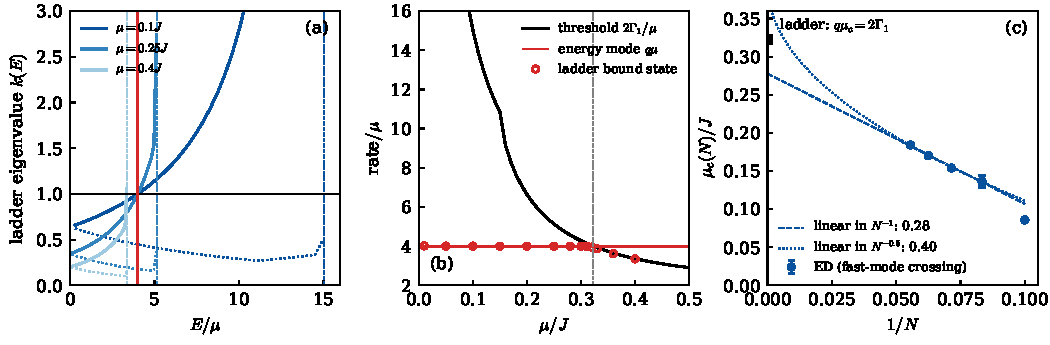
\includegraphics[width=\textwidth]{../figs/fig1_v2.pdf}
\caption{(a) Leading (solid) and subleading (dotted) eigenvalues of the singlet ladder kernel in the exchange-antisymmetric sector versus trial decay rate $E$ ($q=4$, $S=100$). Bound states satisfy $k(E)=1$ (horizontal line). Dashed verticals: thresholds $2\Gamma_1$. Red vertical: $E=q\mu$. (b) Singlet bound-state rates (circles), the exact energy mode $q\mu$ (red) and the threshold $2\Gamma_1/\mu$ from Eq.~\eqref{eq:KB} (black). Dashed: $\mu_c=0.323J$. Above $\mu_c$ the circles are threshold-bound roots that converge to $2\Gamma_1$ as $S\to\infty$. (c) Finite-$N$ crossing $\mu_c(N)$, defined as the coupling at which the slowest fast-sector mode (energy-diagonal weight $<1/2$) reaches $q\mu$, from ED (mean $\pm$ standard error over 3--6 realizations). Lines: linear fits in $1/N$ and $1/\sqrt N$ for $N\ge12$. Square: ladder value.}
\label{fig:ladder}
\end{figure*}

\section{Finite-$N$ crossing with mode identification}
\label{sec:muc}

At finite $N$ we diagonalize $\Lc$ on $\mathrm{span}\{\openone,H\}^\perp$ with a deflated Arnoldi method, as Eq.~\eqref{eq:L} prescribes. We classify each eigenvector by its energy-diagonal weight $w=\|\mathcal D(X)\|^2/\|X\|^2$, where $\mathcal D$ dephases in the energy eigenbasis of each parity block. We define $\mu_c(N)$ as the coupling at which the slowest mode with $w<1/2$ reaches $q\mu$. At this point the slowest mode on $\mathrm{span}\{\openone,H\}^\perp$ has rate $(4.00\pm0.02)\mu$ and $w\le0.15$ for every realization and every $N$ studied. The crossing is thus between the energy mode and a coherence, and no secular mode intervenes. At smaller $\mu$ we observe intermediate weights ($0.2<w<0.8$). These indicate finite-$N$ hybridization between the higher secular modes and the coherences, but they do not affect the crossing.

The crossing grows monotonically with $N$: $\mu_c/J=0.086(3)$, $0.137(8)$, $0.154(2)$, $0.170(1)$ and $0.184(2)$ for $N=10$--$18$ [Fig.~\ref{fig:ladder}(c)]. Extrapolations for $N\ge12$ give $0.28J$ (linear in $1/N$) and $0.40J$ (linear in $1/\sqrt N$), which bracket the ladder value $0.323J$. The data do not fix the extrapolation form, and we do not claim quantitative finite-$N$ confirmation. The slow drift has a natural origin. At finite $N$ the fast branch starts at $N\mu/2$ for $\mu\to0$ and approaches $2\Gamma_1$ only once $N\mu$ greatly exceeds the intrinsic rate. Its value at the crossing is therefore not yet the large-$N$ resonance. The fixed-$\mu$ rates show the same behavior: at $\mu/J=0.4,0.6,0.8$, quadratic extrapolations in $1/N$ of the slowest fast rate give $1.38,1.63,1.93J$, compared with $2\Gamma_1=1.35,1.59,1.90J$.

\section{Relation to previous gap analyses}

Reference~\cite{Zheng2026} computed the gap in the block of opposite parity to the steady state, i.e., among odd operators. That block contains the fermion Green's functions but not $H$. The authors found real ``intruder'' eigenvalues tied to SYK eigenstates and argued that these lose importance as $N\to\infty$, because their number scales as the Hilbert-space dimension while the full spectrum scales as its square. This is consistent with our results. A vanishing fraction of exact modes does not affect the two-point decay rate, but a single exact mode bounds the gap of the even sector, where the physical density matrix lives. Reference~\cite{Zheng2026} also reported that a first-order dynamical transition of the dissipative Loschmidt echo turns into a crossover near $\mu\simeq0.3J$, which they attribute to a proliferation of exceptional points. This value is close to our $\mu_c=0.323J$. We have not established whether the two are related. The echo is a trace over the full operator space and is dominated by the bulk of the spectrum, whereas $\mu_c$ concerns its slowest edge. Similarly, the transitions in the dissipative form factor~\cite{Kawabata2023} concern bulk spectral statistics rather than the gap. The exceptional point $\mu_{\rm EP}\simeq0.16J$ of the fermion Green's function, where the ``$\mu_c\approx0.15$'' of Ref.~\cite{Garcia2023} sits, is likewise distinct from $\mu_c$.

\section{Discussion}

Earlier work established the exact energy mode~\cite{Garcia2026} and the finite anomalous decay of fermion correlations~\cite{Garcia2023,Kulkarni2022}. Anomalous relaxation of two-point functions also appears in an integrable, disorder-free SYK variant~\cite{Ozaki2026}, so it is not specific to chaos. Here we determine how the energy mode competes with the rest of the even spectrum, which makes the conservation-law caveat of Ref.~\cite{Yoshimura2024} quantitative for this model. The answer has three parts. In the slow sector, $H$ is the slowest mode for $N\ge10$. In the fast sector, the large-$N$ ladder contains no collective mode below the two-fermion continuum other than $H$ itself. The two branches cross at $q\mu_c=2\Gamma_1(\mu_c)$. Below $\mu_c$, relaxation is two-stage, and the gap no longer reflects the relaxation of generic observables~\cite{MoriShirai2020}: coherences decay at a rate that remains finite as $\mu\to0$ (at large $N$), while the energy relaxes at $q\mu$. The reflection of $H$ as a bound state of the four-point ladder ties the exact Lindbladian mode to the Keldysh-wormhole description of Ref.~\cite{Garcia2023}. There it corresponds to a normalizable fluctuation of the boundary energy on the doubled contour.

Our conclusions have clear limits. The absence of other bound states is numerical: it holds on the grids and box sizes we used, and it is not a proof. The finite-$N$ crossing is consistent with the ladder value but does not pin it down. The approach of the secular rates to the Ornstein-Uhlenbeck values $\lambda_k=k$ is a trend, not a result. Beyond SYK, the mechanism requires a Hamiltonian that is an eigenvector of the dissipator and has no conserved quantity of lower weight. As the small-$N$ and XXZ examples show, that second condition cannot be assumed. Natural extensions are an analytic treatment of the large-$q$ ladder, where the Liouville solution should make the bound-state condition explicit, and the double-scaled limit~\cite{Berkooz2019,Lin2022}.

\section*{Numerical methods}

ED uses Jordan-Wigner Majoranas and the block structure of even operators in the parity basis. Leading eigenvalues on $\mathrm{span}\{\openone,H\}^\perp$ are computed with shift-deflated Arnoldi iteration (tolerance $10^{-7}$). Full diagonalization was used for $N\le12$. First-order rates are obtained by diagonalizing $\hat n$ within each Bohr-frequency block (tolerance $10^{-7}$). Eq.~\eqref{eq:KB} is integrated with a second-order predictor-corrector scheme ($\delta t=0.004/J$), and $z_1$ is obtained from the Laplace-transformed kernel. The ladder kernel is applied matrix-free by FFT convolution on $[-S,S]$ with $\delta t=0.05/J$, using $S=20$--$450/J$. Leading eigenvalues in the exchange-antisymmetric sector are computed by Arnoldi iteration, and roots of $k(E)=1$ are bracketed by tracking eigenvalue branches. Code and data are available from the author.

\begin{thebibliography}{99}
\bibitem{Kessler2012} E.~M. Kessler, G. Giedke, A. Imamoglu, S.~F. Yelin, M.~D. Lukin, and J.~I. Cirac, Phys.\ Rev.\ A \textbf{86}, 012116 (2012).
\bibitem{Minganti2018} F. Minganti, A. Biella, N. Bartolo, and C. Ciuti, Phys.\ Rev.\ A \textbf{98}, 042118 (2018).
\bibitem{Prosen2002} T. Prosen, J.\ Phys.\ A \textbf{35}, L737 (2002).
\bibitem{Mori2024} T. Mori, Phys.\ Rev.\ B \textbf{109}, 064311 (2024).
\bibitem{Jacoby2025} J.~A. Jacoby, D.~A. Huse, and S. Gopalakrishnan, Phys.\ Rev.\ B \textbf{111}, 104303 (2025).
\bibitem{Zhang2026} T. Zhang, X. Nie, and C. von Keyserlingk, Phys.\ Rev.\ Research \textbf{8}, 033186 (2026).
\bibitem{SY1993} S. Sachdev and J. Ye, Phys.\ Rev.\ Lett.\ \textbf{70}, 3339 (1993).
\bibitem{Kitaev2015} A. Kitaev, talks at KITP (2015).
\bibitem{MS2016} J. Maldacena and D. Stanford, Phys.\ Rev.\ D \textbf{94}, 106002 (2016).
\bibitem{Kulkarni2022} A. Kulkarni, T. Numasawa, and S. Ryu, Phys.\ Rev.\ B \textbf{106}, 075138 (2022).
\bibitem{Garcia2023} A.~M. Garc\'ia-Garc\'ia, L. S\'a, J.~J.~M. Verbaarschot, and J.~P. Zheng, Phys.\ Rev.\ D \textbf{107}, 106006 (2023).
\bibitem{MQ2018} J. Maldacena and X.-L. Qi, arXiv:1804.00491.
\bibitem{Yang2025} T.-H. Yang and D.~A. Abanin, Phys.\ Rev.\ B \textbf{112}, 094304 (2025).
\bibitem{Teretenkov2024} A. Teretenkov and O. Lychkovskiy, Phys.\ Rev.\ B \textbf{110}, L241105 (2024).
\bibitem{Garcia2026} A.~M. Garc\'ia-Garc\'ia, Z. Lu, L. S\'a, and J.~J.~M. Verbaarschot, Phys.\ Rev.\ E \textbf{113}, 024116 (2026).
\bibitem{Garcia2024} A.~M. Garc\'ia-Garc\'ia, J.~J.~M. Verbaarschot, and J.~P. Zheng, arXiv:2403.12359.
\bibitem{Schuster2023} T. Schuster and N.~Y. Yao, Phys.\ Rev.\ Lett.\ \textbf{131}, 160402 (2023).
\bibitem{Bhattacharjee2023} B. Bhattacharjee, X. Cao, P. Nandy, and T. Pathak, J.\ High Energy Phys.\ 03 (2023) 054.
\bibitem{Liu2024} C. Liu, R. Meyer, and Z.-Y. Xian, J.\ High Energy Phys.\ 08 (2024) 092.
\bibitem{Yoshimura2024} T. Yoshimura and L. S\'a, Nat.\ Commun.\ \textbf{15}, 9808 (2024).
\bibitem{Cai2013} Z. Cai and T. Barthel, Phys.\ Rev.\ Lett.\ \textbf{111}, 150403 (2013).
\bibitem{Barthel2022} T. Barthel and Y. Zhang, Phys.\ Rev.\ A \textbf{105}, 052224 (2022).
\bibitem{MoriShirai2020} T. Mori and T. Shirai, Phys.\ Rev.\ Lett.\ \textbf{125}, 230604 (2020).
\bibitem{Macieszczak2016} K. Macieszczak, M. Gu\c{t}\u{a}, I. Lesanovsky, and J.~P. Garrahan, Phys.\ Rev.\ Lett.\ \textbf{116}, 240404 (2016).
\bibitem{Zheng2026} J.~P. Zheng, J. Dukelsky, R.~A. Molina, and A.~M. Garc\'ia-Garc\'ia, Phys.\ Rev.\ D \textbf{113}, 066018 (2026).
\bibitem{Kawabata2023} K. Kawabata, A. Kulkarni, J. Li, T. Numasawa, and S. Ryu, Phys.\ Rev.\ B \textbf{108}, 075110 (2023).
\bibitem{Ozaki2026} S. Ozaki, H. Yoshida, and H. Katsura, arXiv:2606.08079.
\bibitem{Liu2026} X. Liu and A.~M. Garc\'ia-Garc\'ia, arXiv:2608.27897.
\bibitem{Pelliconi2026} P. Pelliconi, B. Lapierre, and S. Ryu, arXiv:2608.19310.
\bibitem{Nosaka2020} T. Nosaka and T. Numasawa, arXiv:2009.10759.
\bibitem{Berkooz2019} M. Berkooz, M. Isachenkov, V. Narovlansky, and G. Torrents, J.\ High Energy Phys.\ 03 (2019) 079.
\bibitem{Lin2022} H.~W. Lin, J.\ High Energy Phys.\ 11 (2022) 060.
\end{thebibliography}

\end{document}
